\begin{center}
  \normalsize{\cyr{\textbf{№3.2}}}
\end{center}

\begin{figure}[h!]
  \centering
  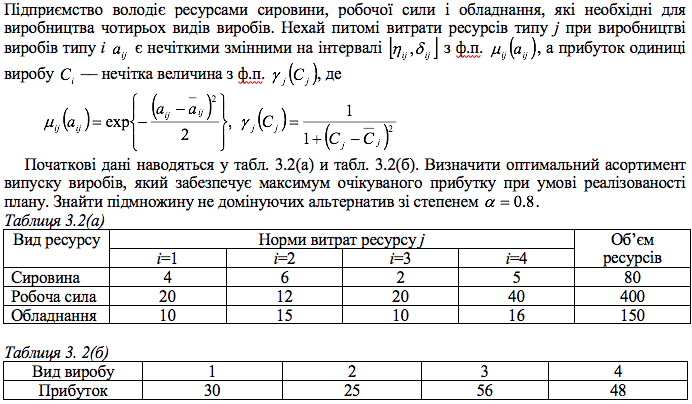
\includegraphics[width=13.8cm]{3_2.png}
  \centering
\end{figure}

Математична модель: $x_{j}$ продукт $j$
\Code{
max \quad   \sum_i^4\  C_{j} x_{j} \qquad  \text{Обмеження} \quad  \sum_{j=1}^3 a_{ij}  x_{j} \leqslant b_j
}

\begin{multicols}{2}
  $$\mu(a_{ij}) \geqslant 0.8  $$

  $$ \exp\{ - \dfrac{(a_{ij}-\overline{a}_{ij})^2}{2} \} \geqslant 0.8 $$
  $$- \dfrac{(a_{ij}-\overline{a}_{ij})^2}{2} \geqslant \ln{0.8} $$
  $$ (a_{ij}-\overline{a}_{ij})^2 \leqslant -2 \ln{0.8} $$
  $$ (a_{ij}-\overline{a}_{ij})^2 \leqslant 2 \ln{\dfrac{1}{0.8}} $$
  $$|a_{ij}-\overline{a}_{ij}| \leqslant \sqrt{2\ln{\dfrac{5}{4}}} $$
  $$ \overline{a}_{ij} - \sqrt{2 \ln{\dfrac{5}{4}}} \leqslant a_{ij} \leqslant \overline{a}_{ij} + \sqrt{ 2 \ln{\dfrac{5}{4}}}$$


  \columnbreak
  $$\gamma(C_{ij}) \geqslant 0.8 $$

  $$\dfrac{1}{1+(C_{ij}-\overline{C}_{ij})^2} \geqslant 0.8$$
  $$\dfrac{1}{0.8} \geqslant 1+(C_{ij}-\overline{C}_{ij})^2$$
  $$\dfrac{1}{0.8} - 1 \geqslant (C_{ij}-\overline{C}_{ij})^2$$
  $$\dfrac{1}{4} \geqslant (C_{ij}-\overline{C}_{ij})^2$$
  $$\dfrac{1}{2} \geqslant |C_{ij}-\overline{C}_{ij}|$$
  $$C_{ij} - \dfrac{1}{2} \leqslant C_{ij} \leqslant C_{ij} + \dfrac{1}{2}$$

\end{multicols}


\begin{multicols}{2}

  \Title{Задача песиміста}

  \Code{
    max \quad \sum_{i=1}^4( \overline{C}_{i} - \dfrac{1}{2} ) x_{j}
  }

  \Title{Обмеження}
  \Code{
    \sum_{j=1}^3( \overline{a}_{ij} + \sqrt{2 \ln{\dfrac{5}{4}}} ) x_{j} \leqslant b_j
  }

  \columnbreak

  \Title{Задача оптиміста}
  \Code{
    max \quad \sum_{i=1}^4( \overline{C}_{i} + \dfrac{1}{2} ) x_{j}
  }

  \Title{Обмеження}
  \Code{
    \sum_{j=1}^3( \overline{a}_{ij} - \sqrt{2 \ln{\dfrac{5}{4}}} ) x_{j} \leqslant b_j
  }


\end{multicols}
